%!TEX root = ../crux-sigconf.tex

\section{Preliminaries}
\label{sec:prelims}
We formalize the problem of crowdsourced entity extraction over structured domains. %First, we define the notion of a {\em structured domain}. We continue by describing entity extraction queries and interfaces over structured domains, along with the response and cost model for these queries. 

\subsection{Structured Data Domains}
\label{sec:data-domain}

Let $\domain$ be a data domain described by a set of discrete attributes $\attributes = \{A_1, A_2, \dots, A_d\}$. Let $dom(A_i)$ denote the domain of each attribute $A_i  \in \attributes$. 
Each attribute $A_i$ can also be hierarchically organized. 
Consider Eventbrite~(\url{www.eventbrite.com}), 
an online event aggregator, that uses crowdsourcing 
to compile a directory of events, such as political rallies and concerts. Events are fully described by their location, type, date and category. Here, entities in the data domain $\domain$ correspond to events. The attributes describing the entities in $\domain$ are $\attributes = \{$``Event Type'', ``Location'', ``Date''$\}$, with ``Location'' and ``Date'' being hierarchically organized.

The domain $\domain$ can be viewed as a {\em poset}, i.e., a partially ordered set, corresponding to the cross-product of all available hierarchies\footnote{Note that $\domain$ is not a lattice since there is no unique infimum.}. Part of the poset corresponding to the previous example is shown in \Cref{fig:eventslattice}. We denote the poset for a domain $\domain$ as $\hierarchy$. As shown in \Cref{fig:eventslattice}, nodes in the poset correspond to configurations where only a subset of the attributes in $\attributes$ are specified while others are allowed to take any value. For example the root of the poset $\{\}$ has no specified attributes, corresponding to queries of the form ``list an event''. Nodes at lower levels, such as $\{X1\}$ and $\{C1\}$, correspond to queries where the event type and location are specified respectively. 

\begin{figure}
	\begin{center}
	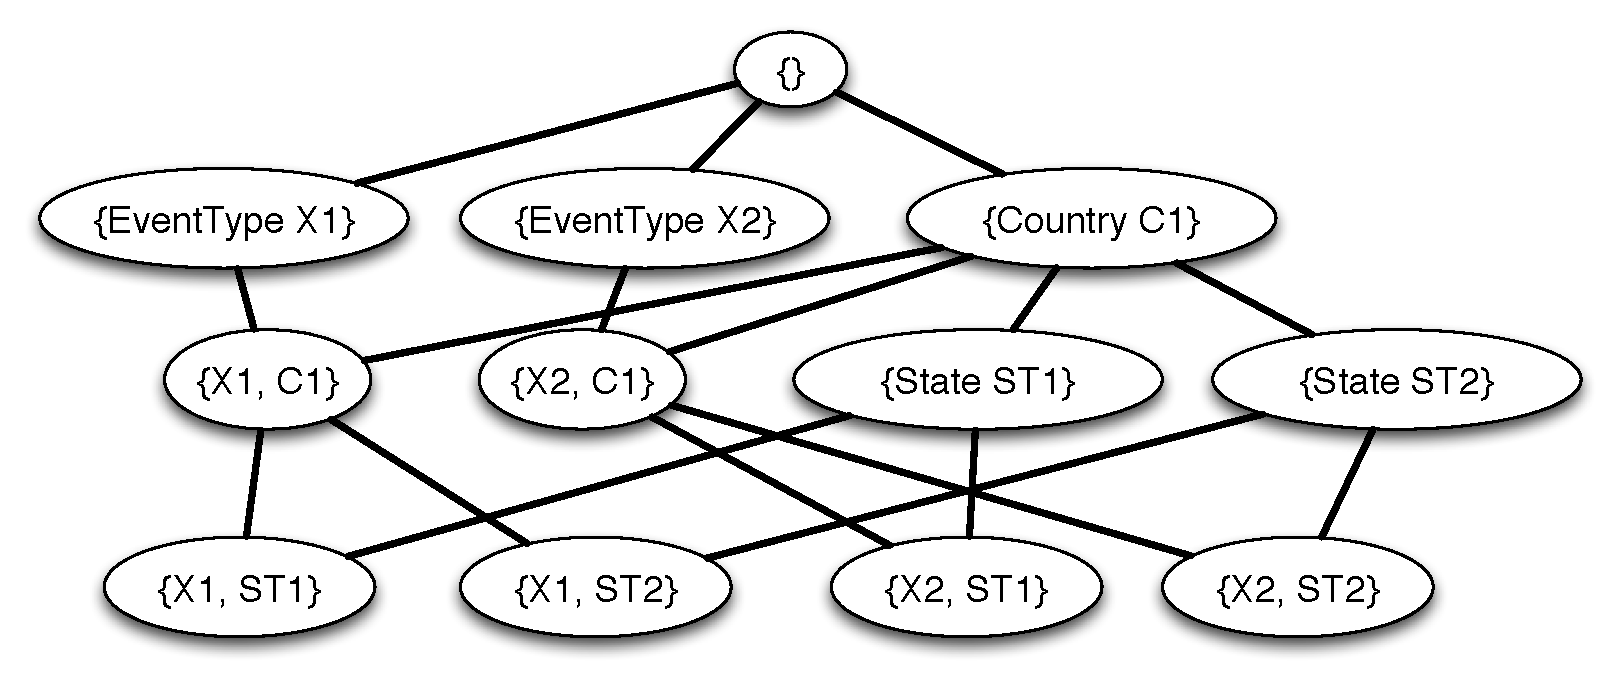
\includegraphics[clip,scale=0.25]{figs/eventsExLattice.eps}
		\vspace{-5pt}
	\caption{Part of the poset for the domain of Eventbrite.}
	\label{fig:eventslattice}
	\vspace{-5pt}
	\end{center}
\end{figure}

\subsection{Entities and Entity Extraction Queries}
\label{sec:queries}

\stitle{Entities.} Our goal is to extract entities from domain $\domain$. Each entity $e$ can be uniquely associated with one of the leaf nodes in the hierarchy $\hierarchy$; that is, there is a unique combination of attribute values $A_1, \ldots, A_d$ characterizing each entity. For example, in Eventbrite, each event is of a specific type, takes place in a specific city, and on a specific day. 
\iftr
Note that our techniques do not fundamentally depend on this assumption and we expect them to work well even if it were not true, but some of the analytical results may not hold in that case.
\fi

\stitle{Queries.} We focus on {\em generalized extraction queries} that can be issued to crowd workers. A query $q^v$ is said to be associated with a node $v \in \hierarchy$ when $q^v$ contains predicates that correspond to the value combination for $\attributes$ associated with $v$. For example, if we consider the poset in \Cref{fig:eventslattice} a query for node $\{X1\}$ has a predicate $EventType = X1$. Hence, workers are required to provide events that satisfy this predicate.

There are three types of queries $q^v$: (i) {\em Single entity queries} where workers are required to provide only ``one more'' entity matching the predicates of the query, (ii) {\em queries of size k} where workers are asked to provide $k$ distinct entities for a query $q^v$, and (iii) {\em exclude list queries} where workers are additionally provided with a list $E$ of $l$ entities that have already been extracted and they are required to provide $k$ distinct entities that are not present in the exclude list. It is easy to see that the last variation generalizes the previous two. Therefore, in the remainder of the paper, we will only consider queries using the third configuration. We refer to these queries as {\em generalized} queries. To describe a generalized query, we use the notation $q^v(k,E)$ denoting a query of size $k$ with an exclude list $E$ of length $l$ that is associated with node $v \in \hierarchy$. We denote the configuration for a query as $(k,l,v)$.

\subsection{Query Response} 
We consider a querying interface that asks human workers to not only list entities but to also provide, for each entity, the values for its attributes in $\attributes$ that are not specified in the predicates of $q$. For example, if the query is ``list one concert in Manhattan, New York'', with $k = 1, E = \emptyset$, the worker gives us one concert in Manhattan, New York, but also gives us the day on which the concert will take place (here, the missing, unspecified attribute) and the type of concert, i.e., rock concert. If the query is ``a concert in the US'', with $k = 1, E = \emptyset$, the human worker gives us one concert in the US, but also gives the day on which the concert will take place, as well as the specific city. If less than $k$ entities are present in the underlying population, workers have the flexibility to report either an empty answer or a smaller number of entities. 
\iftr
The above interface can trivially support queries that either require workers to list entities leveraging their own domain knowledge or queries that restrict workers to specific data sources such as raw text or raw web-pages as illustrated in our pilot experiment in Section~\ref{sec:intro}.
\fi

While getting additional attribute values for entities is not strictly necessary, this information allows us to assign an extracted entity to all relevant nodes in $\hierarchy$. 
\iftr
Without this, it is difficult to effectively collect information about the entity population associated with each node in the poset. 
\fi
Furthermore, in most practical applications, it is useful to get the values of the missing attributes to organize and categorize the extracted entities better. Similar query interfaces that ask users to fully specify the attributes of entities have been proposed in recent work~\cite{quinn:2014}.  That said, our techniques still apply even if workers do not provide
all attributes: in such a setting, entities will be assigned to interior nodes but not to leaves.

%\subsection{Noisy and Duplicate Answers} 
Often, workers unwittingly provide the same entity, resulting in duplicates. Resolving duplicates during extraction is crucial for two reasons: (i) they are used to estimate the completeness of extracted entities, and thus, reason about the gain of additional queries, and (ii) they can be used to resolve erroneous values for the attributes of the extracted entities. In practice, standard entity resolution and data fusion techniques~\cite{getoor:kdd13} can be used to address this problem. Given that we obtain information about several attributes of entities from the crowd, we can apply simple rules that match the entity attribute values 
\iftr (e.g., using string similarities or other measure such as Jaccard similarity)
\fi 
to detect duplicates and resolve erroneous values. Additional worker quality detection techniques that consider limited ground truth data~\cite{donmez-learning-inference} can be used to determine the accuracy of workers. During our experiments, we found that simple data fusion techniques were sufficient to resolve noisy labels and duplicates. 
So, for this paper, we focus on devising near-optimal adaptive crowd querying strategies for entity extraction. 

\iftr
Finally, answers are expected to be duplicated across workers, who may also specify or extract an entity incorrectly. Resolving duplicate entities during extraction is crucial as this information is later used to estimate characterize the completeness of extracted entities, and thus, reason about the gain of additional queries.  Extraction errors can be resolved by leveraging the presence of duplicate information and by applying de-duplication and entity resolution techniques. At a high-level one can use an entity resolution or string similarity (e.g., Jaccard coefficient) algorithm to identify duplicate entities. Furthermore, the additional attributes for each entity, can be used to further ascertain similarity of entities. We refer the user to Getoor and Machanavajjhala~\cite{getoor:kdd13} for an overview of entity resolution techniques. Finally, standard truth discovery techniques can be used to identify the correct attribute values for entities. Nevertheless entity resolution and truth discovery are orthogonal problems and not the focus of this paper. In our experiments on real datasets, we found that there were no cases where humans introduced errors to the attribute values of extracted entities. Only minor errors (e.g., misspelled entity names) were detected and fixed manually. \fi

\subsection{Query Cost} 
In a typical crowdsourcing marketplace, tasks have different costs based on their difficulty. While our algorithms works with any cost function, we consider a cost function $c(\cdot)$ that obeys the following properties:  (a) given a query with fixed size, its cost should increase (or remain the same) as the size of its exclude list should increase, (b) given a query with a fixed exclude list size, its cost should increase (or remain the same) as the number of requested answer increases, and (c) given a query with fixed size and exclude list size, its cost should increase (or remain the same) as the query contains more predicates, i.e., it corresponds to nodes $v$ at the lower-levels of $\hierarchy$. The cost function is fixed upfront by the interface-designer based on the amount of work involved.

%{\stitle{Note on Assumptions.} The various assumptions made above are not essential to our framework, and our techniques are applicable even if those do not hold, but they may not be as effective. For example, if an entity returned by a user is underspecified, then it will only be assigned to an interior node of the poset and not to the appropriate leaf. Therefore, it will not be used to improve the estimates for that leaf. Similarly, if we are not able to identify duplicates, the two entities would be treated as different, potentially affecting the gain estimates. We plan to formally to investigate the effects of such errors in future work.}